\documentclass[11pt,a4paper]{article}
\usepackage{amsmath}\usepackage{amssymb}\usepackage[table]{xcolor}
\usepackage{tabularx}\usepackage{multirow}\usepackage{geometry}
\usepackage{enumitem}\usepackage{parskip}\usepackage{titlesec}
\usepackage{tocloft}\usepackage[most]{tcolorbox}
\usepackage{tikz}\usepackage{pgfplots}\pgfplotsset{compat=1.18}\usetikzlibrary{arrows.meta,calc,positioning,shapes.geometric,patterns}
\geometry{margin=2.5cm}
\titleformat{\section}{\large\bfseries}{}{0em}{}
\setlength{\cftbeforesecskip}{6pt}
\definecolor{q1color}{HTML}{D6EAF8}\definecolor{q2color}{HTML}{D5F5E3}
\definecolor{q3color}{HTML}{FDEBD0}\definecolor{q4color}{HTML}{F9E79F}
\definecolor{q5color}{HTML}{E8DAEF}\definecolor{q6color}{HTML}{FADBD8}
\definecolor{q7color}{HTML}{D1F2EB}\definecolor{q8color}{HTML}{FCF3CF}
\definecolor{q9color}{HTML}{EBDEF0}\definecolor{q10color}{HTML}{F5EEF8}
\newenvironment{mstab}[1]{%
  {\color{#1!75!black}\nobreak Mark Scheme}\par\nopagebreak\smallskip
  \arrayrulecolor{#1!70!black}\renewcommand{\arraystretch}{1.3}%
  \tabularx{\textwidth}{|>{\columncolor{#1!12}\raggedright\arraybackslash}p{1.9cm}|>{\columncolor{#1!12}}X|>{\columncolor{#1!12}\centering\arraybackslash}p{1.1cm}|}%
  \hline\rowcolor{#1!45} Question & Answer & Marks \\ \hline}{%
  \endtabularx\arrayrulecolor{black}\par\medskip}
\newtcolorbox{ansbox}[1]{colback=#1!8,colbacktitle=#1!30,colframe=#1!70!black,coltitle=black,fonttitle=\normalfont,title=Worked Solution,boxrule=0.6pt,arc=2mm,left=4pt,right=4pt,top=4pt,bottom=4pt,breakable}
\newcommand{\topiclabel}[1]{\hfill\normalfont\small\itshape\textcolor{black!55}{#1}}
\newcommand{\examq}[4]{\section[#1 - Q#2]{#1 - Q#2 - #3 - #4}}
\begin{document}
\begin{center}
  {\LARGE \textbf{Cambridge O Level Additional Mathematics 4037/12/M/J/16}}\\[6pt]
  {\large May/June 2016 -- Mark Scheme \& Worked Solutions}
\end{center}
\bigskip

% ===================================================== Q1
\examq{4037/12/M/J/16}{1}{Excluded from the present curriculum}{4}
\begin{mstab}{q1color}
 & $Y\subset X$ or $Y\subseteq X$ only & B1 \\ \hline
\multirow{-2}{1.9cm}{1(a)} & $Y\cap Z=\varnothing$ or $\{\ \}$ only & B1 \\ \hline
 & Diagram (i): $(A\cup B)\cap C$ correctly shaded & B1 \\ \hline
\multirow{-2}{1.9cm}{1(b)} & Diagram (ii): $A\cup(B\cap C)$ correctly shaded & B1 \\ \hline
\end{mstab}
\begin{ansbox}{q1color}
\textbf{(a)} Every multiple of 10 is also a multiple of 5, so $Y$ is a subset of $X$:
\[ \boxed{Y\subset X} \]
$Z=\{\pi,\ 2,\ \mathrm{e}\}$. The only integer in $Z$ is $2$, and $2$ is not a multiple of 10, so $Y$ and $Z$ have no elements in common:
\[ \boxed{Y\cap Z=\varnothing} \]

\textbf{(b)} \textbf{Diagram (i)} $(A\cup B)\cap C$: shade the parts of circle $C$ that also lie inside $A$ or inside $B$.

\textbf{Diagram (ii)} $A\cup(B\cap C)$: shade the whole of circle $A$ together with the overlap of $B$ and $C$.
\end{ansbox}

% ===================================================== Q2
\examq{4037/12/M/J/16}{2}{Binomial Theorem}{5}
\begin{mstab}{q2color}
2(i) & $32-\dfrac{20}{x}+\dfrac{5}{x^2}$ \newline \textit{B1 for each correct term -- must be integers} & B3 \\ \hline
 & $\left(-\dfrac{20}{x}\right)\times 4x+32\times 3$ \newline \textit{M1 for $\left(\text{their}\,(-20)\right)\times 4+\left(\text{their}\,32\right)\times 3$} & M1 \\ \hline
\multirow{-2}{1.9cm}{2(ii)} & $=16$ \newline \textit{Accept $16x^0$} & A1 \\ \hline
\end{mstab}
\begin{ansbox}{q2color}
\textbf{(i)} Expand $\left(2-\dfrac{1}{4x}\right)^5$ using the binomial theorem:
\[ \left(2-\frac{1}{4x}\right)^5=2^5+\binom{5}{1}2^4\left(-\frac{1}{4x}\right)+\binom{5}{2}2^3\left(-\frac{1}{4x}\right)^2+\cdots \]
\[ =32+5(16)\left(-\frac{1}{4x}\right)+10(8)\left(\frac{1}{16x^2}\right)+\cdots=32-\frac{20}{x}+\frac{5}{x^2}+\cdots \]
\[ \boxed{a=32,\qquad b=-20,\qquad c=5} \]

\textbf{(ii)} In $\left(2-\dfrac{1}{4x}\right)^5(3+4x)$, the term independent of $x$ comes from $32\times 3$ and from $\left(-\dfrac{20}{x}\right)\times 4x$:
\[ 32\times 3+\left(-\frac{20}{x}\right)(4x)=96-80=\boxed{16} \]
\end{ansbox}

% ===================================================== Q3
\examq{4037/12/M/J/16}{3}{Vectors in Two Dimensions}{6}
\begin{mstab}{q3color}
 & $\mathbf{b}-\mathbf{c}=\begin{pmatrix}6\\-2\end{pmatrix}$ \newline \textit{may be implied by further correct working} & B1 \\ \hline
 & $y^2+4=36+4$ \newline \textit{M1 for one correct attempt at using the modulus} & M1 \\ \hline
\multirow{-3}{1.9cm}{3(i)} & $y=\pm 6$ & A1 \\ \hline
 & $\lambda+4=2\mu$ \ or \ $-4\lambda+24=7\mu$ \newline \textit{B1 for one correct equation in $\mu$ and $\lambda$} & B1 \\ \hline
 & $\lambda-4=-\mu$ \ or \ $8\lambda-8=\mu$ \newline \textit{B1 for a second correct equation in $\mu$ and $\lambda$} & B1 \\ \hline
\multirow{-3}{1.9cm}{3(ii)} & leading to $\lambda=\dfrac{4}{3}$, \ $\mu=\dfrac{8}{3}$ oe \newline \textit{allow 1.33 and 2.67 or better} \newline \textit{DB1 for both, must have both previous B marks} & DB1 \\ \hline
\end{mstab}
\begin{ansbox}{q3color}
$\mathbf{b}=\begin{pmatrix}1\\3\end{pmatrix}$, \ $\mathbf{c}=\begin{pmatrix}-5\\5\end{pmatrix}$, and $\mathbf{a}$ has components $y$ and $2$.

\textbf{(i)}
\[ \mathbf{b}-\mathbf{c}=\begin{pmatrix}1-(-5)\\3-5\end{pmatrix}=\begin{pmatrix}6\\-2\end{pmatrix},\qquad |\mathbf{b}-\mathbf{c}|^2=36+4=40 \]
$|\mathbf{a}|=|\mathbf{b}-\mathbf{c}|$, so
\[ y^2+2^2=36+4 \;\Rightarrow\; y^2=36 \;\Rightarrow\; \boxed{y=\pm 6} \]

\textbf{(ii)} $\lambda(\mathbf{b}+\mathbf{c})+4(\mathbf{b}-\mathbf{c})=\mu(2\mathbf{b}-\mathbf{c})$. Since $\mathbf{b}$ and $\mathbf{c}$ are not parallel, compare coefficients of $\mathbf{b}$ and of $\mathbf{c}$:
\[ \mathbf{b}:\ \lambda+4=2\mu \qquad\qquad \mathbf{c}:\ \lambda-4=-\mu \]
Adding $2\times$(second) to the first eliminates $\mu$:
\[ \lambda+4+2(\lambda-4)=0 \;\Rightarrow\; 3\lambda=4 \;\Rightarrow\; \lambda=\frac{4}{3},\qquad \mu=4-\lambda=\frac{8}{3} \]
(Using components instead: $\mathbf{b}+\mathbf{c}=\begin{pmatrix}-4\\8\end{pmatrix}$, $2\mathbf{b}-\mathbf{c}=\begin{pmatrix}7\\1\end{pmatrix}$ give $-4\lambda+24=7\mu$ and $8\lambda-8=\mu$, with the same solution.)
\[ \boxed{\lambda=\frac{4}{3},\qquad \mu=\frac{8}{3}} \]
\end{ansbox}

% ===================================================== Q4
\examq{4037/12/M/J/16}{4}{Quadratic Functions \textperiodcentered\ Indices \& Surds}{6}
\begin{mstab}{q4color}
 & \textit{You must be convinced that a calculator is not being used.} \newline $\left(4+\sqrt{5}\right)x^2+\left(2-\sqrt{5}\right)x-1=0$ \newline $x=\dfrac{-\left(2-\sqrt{5}\right)\pm\sqrt{\left(2-\sqrt{5}\right)^2+4\left(4+\sqrt{5}\right)}}{2\left(4+\sqrt{5}\right)}$ \newline \textit{M1 for use of quadratic formula (allow one sign error), allow $b^2=9-4\sqrt{5}$} & M1 \\ \hline
 & \textit{A1 all correct} & A1 \\ \hline
 & $x=\dfrac{-\left(2-\sqrt{5}\right)\pm\sqrt{9-4\sqrt{5}+16+4\sqrt{5}}}{2\left(4+\sqrt{5}\right)}$ \newline \textit{DM1 for attempt to simplify the discriminant (minimum of 4 terms must be seen in discriminant, 2 terms involving $\sqrt{5}$ and 2 constant terms)} & DM1 \\ \hline
 & $=\dfrac{-\left(2-\sqrt{5}\right)+5}{2\left(4+\sqrt{5}\right)}=\dfrac{3+\sqrt{5}}{2\left(4+\sqrt{5}\right)}$ \newline \textit{A1 for $\dfrac{3+\sqrt{5}}{2\left(4+\sqrt{5}\right)}$ or $\dfrac{3+\sqrt{5}}{8+2\sqrt{5}}$, ignore negative solution if included} & A1 \\ \hline
 & $=\dfrac{\left(3+\sqrt{5}\right)\left(4-\sqrt{5}\right)}{2\left(4+\sqrt{5}\right)\left(4-\sqrt{5}\right)}$ \newline \textit{M1 for attempt to rationalise an expression of the form $\dfrac{a\pm b\sqrt{5}}{c\pm d\sqrt{5}}$ as part of their solution of the quadratic. Must obtain an integer denominator} & M1 \\ \hline
\multirow{-6}{1.9cm}{4} & $=\dfrac{7+\sqrt{5}}{22}$ \newline \textit{Final A1 can only be awarded if all previous marks have been obtained} & A1 \\ \hline
\end{mstab}
\begin{ansbox}{q4color}
Solve $\left(4+\sqrt{5}\right)x^2+\left(2-\sqrt{5}\right)x-1=0$ with the quadratic formula, $a=4+\sqrt{5}$, $b=2-\sqrt{5}$, $c=-1$.

Discriminant:
\[ b^2-4ac=\left(2-\sqrt{5}\right)^2+4\left(4+\sqrt{5}\right)=\left(9-4\sqrt{5}\right)+\left(16+4\sqrt{5}\right)=25 \]
Taking the positive root:
\[ x=\frac{-\left(2-\sqrt{5}\right)+5}{2\left(4+\sqrt{5}\right)}=\frac{3+\sqrt{5}}{2\left(4+\sqrt{5}\right)} \]
Rationalise the denominator using $\left(4+\sqrt{5}\right)\left(4-\sqrt{5}\right)=16-5=11$:
\[ x=\frac{\left(3+\sqrt{5}\right)\left(4-\sqrt{5}\right)}{2\times 11}=\frac{12-3\sqrt{5}+4\sqrt{5}-5}{22} \]
\[ \boxed{x=\frac{7+\sqrt{5}}{22}} \qquad (a=7,\ b=22) \]
\end{ansbox}

% ===================================================== Q5
\examq{4037/12/M/J/16}{5}{Trigonometry}{7}
\begin{mstab}{q5color}
 & $(1-\cos\theta)(1+\sec\theta)=1-\cos\theta+\dfrac{1}{\cos\theta}-\dfrac{\cos\theta}{\cos\theta}$ \newline \textit{M1 for expansion and use of $\sec\theta=\dfrac{1}{\cos\theta}$ consistently, allow one sign error} & M1 \\ \hline
 & $=\sec\theta-\cos\theta=\dfrac{1}{\cos\theta}-\cos\theta=\dfrac{1-\cos^2\theta}{\cos\theta}$ \newline \textit{DM1 for attempt at a single fraction, dependent on first M1} & DM1 \\ \hline
 & $=\dfrac{\sin^2\theta}{\cos\theta}$ & A1 \\ \hline
 & $=\sin\theta\tan\theta$ \ www & A1 \\ \hline
 & \textbf{Alternative method:} \newline $(1-\cos\theta)\left(\dfrac{\cos\theta+1}{\cos\theta}\right)$ \newline \textit{M1 for attempt at a single fraction for second factor and use of $\sec\theta=\dfrac{1}{\cos\theta}$} & M1 \\ \hline
 & $=\dfrac{1-\cos^2\theta}{\cos\theta}$ \newline \textit{DM1 for expansion} & DM1 \\ \hline
 & $=\dfrac{\sin^2\theta}{\cos\theta}$ & A1 \\ \hline
\multirow{-8}{1.9cm}{5(i)} & $=\sin\theta\tan\theta$ \ www & A1 \\ \hline
 & $\sin\theta\tan\theta=\sin\theta$ \newline $\sin\theta(\tan\theta-1)=0$ \newline $\tan\theta=1$, \ $\theta=\dfrac{\pi}{4}$, allow 0.785 or better \newline \textit{B1 for $\theta=\dfrac{\pi}{4}$ from $\tan\theta=1$} & B1 \\ \hline
 & $\sin\theta=0$, \ $\theta=0$ \newline \textit{B1 for $\theta=0$ from $\sin\theta=0$} & B1 \\ \hline
\multirow{-3}{1.9cm}{5(ii)} & $\theta=\pi$ or 3.14 or better \newline \textit{B1 for $\theta=\pi$ from $\sin\theta=0$} & B1 \\ \hline
\end{mstab}
\begin{ansbox}{q5color}
\textbf{(i)} Expand and use $\sec\theta=\dfrac{1}{\cos\theta}$:
\[ (1-\cos\theta)(1+\sec\theta)=1+\frac{1}{\cos\theta}-\cos\theta-\frac{\cos\theta}{\cos\theta}=\frac{1}{\cos\theta}-\cos\theta \]
Write as a single fraction and use $1-\cos^2\theta=\sin^2\theta$:
\[ =\frac{1-\cos^2\theta}{\cos\theta}=\frac{\sin^2\theta}{\cos\theta}=\sin\theta\cdot\frac{\sin\theta}{\cos\theta}=\sin\theta\tan\theta \]
as required.

\textbf{(ii)} Using (i), the equation becomes
\[ \sin\theta\tan\theta=\sin\theta \;\Rightarrow\; \sin\theta(\tan\theta-1)=0 \]
For $0\leqslant\theta\leqslant\pi$:
\[ \sin\theta=0 \;\Rightarrow\; \theta=0,\ \pi \qquad\qquad \tan\theta=1 \;\Rightarrow\; \theta=\frac{\pi}{4} \]
\[ \boxed{\theta=0,\ \frac{\pi}{4},\ \pi} \]
\end{ansbox}

% ===================================================== Q6
\examq{4037/12/M/J/16}{6}{Differentiation \textperiodcentered\ Logarithmic \& Exponential Functions}{5}
\begin{mstab}{q6color}
 & $\dfrac{\mathrm{d}}{\mathrm{d}x}\left(\mathrm{e}^{3x}(4x+1)^{\frac{1}{2}}\right)=\mathrm{e}^{3x}\times\dfrac{1}{2}(4x+1)^{-\frac{1}{2}}\times 4+3\mathrm{e}^{3x}(4x+1)^{\frac{1}{2}}$ \newline \textit{B1 for $r\mathrm{e}^{3x}(4x+1)^{-\frac{1}{2}}$, must be part of a sum, $r=\dfrac{1}{2}$ or $2$ or $\dfrac{1}{2}\times 4$} & B1 \\ \hline
 & \textit{B1 for $s\mathrm{e}^{3x}(4x+1)^{\frac{1}{2}}$, must be part of a sum, $s$ is 1 or 3} & B1 \\ \hline
 & $=\dfrac{2\mathrm{e}^{3x}}{(4x+1)^{\frac{1}{2}}}+3\mathrm{e}^{3x}(4x+1)^{\frac{1}{2}}$ \newline \textit{B1 for all correct, allow unsimplified} & B1 \\ \hline
 & $=\dfrac{\mathrm{e}^{3x}}{(4x+1)^{\frac{1}{2}}}\left(2+12x+3\right)$ \newline \textit{DM1 for $\dfrac{\mathrm{e}^{3x}}{(4x+1)^{\frac{1}{2}}}(a+bx)$, dependent on first 2 B marks, must be using a correct method, collecting terms in the numerator correctly} & DM1 \\ \hline
\multirow{-5}{1.9cm}{6} & $=\dfrac{\mathrm{e}^{3x}}{(4x+1)^{\frac{1}{2}}}(12x+5)$ & A1 \\ \hline
\end{mstab}
\begin{ansbox}{q6color}
Write $\sqrt{4x+1}=(4x+1)^{\frac{1}{2}}$ and use the product rule with the chain rule:
\[ \frac{\mathrm{d}}{\mathrm{d}x}\left(\mathrm{e}^{3x}(4x+1)^{\frac{1}{2}}\right)=\mathrm{e}^{3x}\cdot\frac{1}{2}(4x+1)^{-\frac{1}{2}}\cdot 4+3\mathrm{e}^{3x}(4x+1)^{\frac{1}{2}} \]
\[ =\frac{2\mathrm{e}^{3x}}{\sqrt{4x+1}}+3\mathrm{e}^{3x}\sqrt{4x+1} \]
Put over the common denominator $\sqrt{4x+1}$:
\[ =\frac{\mathrm{e}^{3x}\left[2+3(4x+1)\right]}{\sqrt{4x+1}}=\frac{\mathrm{e}^{3x}(12x+5)}{\sqrt{4x+1}} \]
\[ \boxed{p=12,\qquad q=5} \]
\end{ansbox}

% ===================================================== Q7
\examq{4037/12/M/J/16}{7}{Integration \textperiodcentered\ Trigonometry}{8}
\begin{mstab}{q7color}
 & $\cos 3x=\dfrac{1}{2}$ \newline \textit{M1 for correct attempt to solve the trigonometric equation} & M1 \\ \hline
\multirow{-2}{1.9cm}{7(i)} & $x=\dfrac{\pi}{9}$ or $0.349$, \ allow $0.35$ \ ($20^\circ$) & A1 \\ \hline
7(ii) & $\left(\dfrac{\pi}{3},\ 3\right)$ or $(1.05,\ 3)$, \ $\left(60^\circ,\ 3\right)$ \newline \textit{B1 for each, must be in correct position or in terms of $x=$ and $y=$} & B1B1 \\ \hline
 & $\displaystyle\int_{\frac{\pi}{9}}^{\frac{\pi}{3}}1-2\cos 3x\,\mathrm{d}x=\left[x-\dfrac{2}{3}\sin 3x\right]_{\frac{\pi}{9}}^{\frac{\pi}{3}}$ \newline \textit{M1 for $x\pm a\sin 3x$, attempt to integrate at least one term} & M1 \\ \hline
 & \textit{A1 for correct integration} & A1 \\ \hline
 & $=\dfrac{\pi}{3}-\left(\dfrac{\pi}{9}-\dfrac{2}{3}\times\dfrac{\sqrt{3}}{2}\right)$ \newline \textit{DM1 for correct use of limits from (i) and (ii), must be in radians} & DM1 \\ \hline
\multirow{-4}{1.9cm}{7(iii)} & $=\dfrac{2\pi}{9}+\dfrac{\sqrt{3}}{3}$ oe or $1.28$ & A1 \\ \hline
\end{mstab}
\begin{ansbox}{q7color}
$y=1-2\cos 3x$.

\textbf{(i)} At $A$, $y=0$:
\[ 1-2\cos 3x=0 \;\Rightarrow\; \cos 3x=\frac{1}{2} \;\Rightarrow\; 3x=\frac{\pi}{3} \;\Rightarrow\; x=\frac{\pi}{9} \]
\[ \boxed{A\left(\frac{\pi}{9},\ 0\right)} \]

\textbf{(ii)} $y$ is a maximum when $\cos 3x=-1$, i.e. $3x=\pi$, so $x=\dfrac{\pi}{3}$ and $y=1-2(-1)=3$:
\[ \boxed{B\left(\frac{\pi}{3},\ 3\right)} \]

\textbf{(iii)} The shaded area lies above the $x$-axis from $x=\dfrac{\pi}{9}$ to $x=\dfrac{\pi}{3}$:
\[ \int_{\frac{\pi}{9}}^{\frac{\pi}{3}}\left(1-2\cos 3x\right)\mathrm{d}x=\left[x-\frac{2}{3}\sin 3x\right]_{\frac{\pi}{9}}^{\frac{\pi}{3}} \]
\[ =\left(\frac{\pi}{3}-\frac{2}{3}\sin\pi\right)-\left(\frac{\pi}{9}-\frac{2}{3}\sin\frac{\pi}{3}\right)=\frac{\pi}{3}-\frac{\pi}{9}+\frac{2}{3}\cdot\frac{\sqrt{3}}{2} \]
\[ \boxed{\frac{2\pi}{9}+\frac{\sqrt{3}}{3}\approx 1.28} \]
\end{ansbox}

% ===================================================== Q8
\examq{4037/12/M/J/16}{8}{Straight-Line Graphs \textperiodcentered\ Logarithmic \& Exponential Functions}{8}
\begin{mstab}{q8color}
 & $\lg y=\lg A+x^2\lg b$ & B1 \\ \hline
 & $\lg b=\pm 0.21$ \newline \textit{B1 for $\lg b=\pm 0.21$, may be implied} & B1 \\ \hline
 & $b=0.617$, \ allow $0.62$, $10^{-0.21}$ \newline $\lg A=0.94$, \ allow $0.93$ to $0.95$ & B1 \\ \hline
 & $A=8.71$, \ allow awrt $8.5$ to $8.9$ & B1 \\ \hline
 & \textbf{Alternative method:} \newline $Ab=5.37$ or $10^{0.73}$ \newline $Ab^4=1.259$ or $10^{0.1}$ \newline \textit{B1 for both equations, allow correct to 2 sf} & B1 \\ \hline
 & $b^3=10^{-0.63}$ & B1 \\ \hline
 & $b=0.617$, \ allow $0.62$, $10^{-0.21}$ & B1 \\ \hline
\multirow{-8}{1.9cm}{8(i)} & $A=8.71$, \ allow awrt $8.5$ to $8.9$ & B1 \\ \hline
 & $x=1.5$, \ $x^2=2.25$ \newline \textit{M1 for correct use of graph, $y=\text{their}A\times\text{their}b^{1.5^2}$ or $\lg y=\lg\text{their}A+1.5^2\lg\text{their}b$} & M1 \\ \hline
\multirow{-2}{1.9cm}{8(ii)} & $y=2.93$, \ allow awrt $2.9$ or $3.0$ & A1 \\ \hline
 & $\lg y=0.301$, or $2=8.71\times 0.617^{x^2}$ \newline \textit{M1 for correct use of graph to read off $x^2$, or $2=\text{their}A\left(\text{their}b\right)^{x^2}$ or $\lg 2=\lg\text{their}A+x^2\lg\text{their}b$} & M1 \\ \hline
\multirow{-2}{1.9cm}{8(iii)} & $x=1.74$, \ allow $\sqrt{3}$ or awrt $1.7$, $1.8$ & A1 \\ \hline
\end{mstab}
\begin{ansbox}{q8color}
\textbf{(i)} Take lg of $y=Ab^{x^2}$:
\[ \lg y=\lg A+x^2\lg b \]
This is a straight line in $\lg y$ against $x^2$ with gradient $\lg b$ and intercept $\lg A$. Using $(1,\ 0.73)$ and $(4,\ 0.10)$:
\[ \lg b=\frac{0.10-0.73}{4-1}=-0.21 \;\Rightarrow\; b=10^{-0.21}=\boxed{0.617} \]
\[ \lg A=0.73-(-0.21)(1)=0.94 \;\Rightarrow\; A=10^{0.94}=\boxed{8.71} \]

\textbf{(ii)} $x=1.5$, so $x^2=2.25$:
\[ \lg y=0.94-0.21(2.25)=0.4675 \;\Rightarrow\; y=10^{0.4675}=\boxed{2.93} \]

\textbf{(iii)} $y=2$, so $\lg y=\lg 2=0.301$:
\[ 0.301=0.94-0.21x^2 \;\Rightarrow\; x^2=\frac{0.639}{0.21}=3.04 \;\Rightarrow\; \boxed{x=1.74} \]
\end{ansbox}

% ===================================================== Q9
\examq{4037/12/M/J/16}{9}{Differentiation \textperiodcentered\ Integration}{10}
\begin{mstab}{q9color}
 & $y=\dfrac{2}{3}(3x+10)^{\frac{1}{2}}\ (+c)$ \newline \textit{B1 for $p(3x+10)^{\frac{1}{2}}$ where $p$ is a constant} & B1 \\ \hline
 & \textit{B1 for $\dfrac{2}{3}(3x+10)^{\frac{1}{2}}$ oe unsimplified} & B1 \\ \hline
 & passes through $\left(2,\ -\dfrac{4}{3}\right)$, so $c=-4$ \newline \textit{M1 for attempt to find $c$, must have attempt to integrate, must have the first B1} & M1 \\ \hline
\multirow{-4}{1.9cm}{9(i)} & $y=\dfrac{2}{3}(3x+10)^{\frac{1}{2}}-4$ oe & A1 \\ \hline
 & When $x=5$, \ $y=-\dfrac{2}{3}$ & B1 \\ \hline
 & perpendicular gradient $=-5$ & B1 \\ \hline
 & Equation of normal: $y+\dfrac{2}{3}=-5(x-5)$ \newline \textit{M1 for attempt at the normal using their perpendicular gradient and their $y$ value (but not $y=-\dfrac{4}{3}$ or $-\dfrac{5}{3}$)} & M1 \\ \hline
 & \textit{A1 for correct normal} & A1 \\ \hline
 & When $y=-\dfrac{5}{3}$, \newline \textit{DM1 for use of $y=-\dfrac{5}{3}$ in their normal equation to get as far as $x=\ldots$} & DM1 \\ \hline
\multirow{-6}{1.9cm}{9(ii)} & $x=5.2$ oe & A1 \\ \hline
\end{mstab}
\begin{ansbox}{q9color}
\textbf{(i)} $\dfrac{\mathrm{d}y}{\mathrm{d}x}=(3x+10)^{-\frac{1}{2}}$. Integrate (reverse chain rule, dividing by 3):
\[ y=\frac{(3x+10)^{\frac{1}{2}}}{\frac{1}{2}\times 3}+c=\frac{2}{3}(3x+10)^{\frac{1}{2}}+c \]
Through $\left(2,\ -\dfrac{4}{3}\right)$:
\[ -\frac{4}{3}=\frac{2}{3}\sqrt{16}+c=\frac{8}{3}+c \;\Rightarrow\; c=-4 \]
\[ \boxed{y=\frac{2}{3}(3x+10)^{\frac{1}{2}}-4} \]

\textbf{(ii)} At $x=5$:
\[ y=\frac{2}{3}\sqrt{25}-4=\frac{10}{3}-4=-\frac{2}{3},\qquad \frac{\mathrm{d}y}{\mathrm{d}x}=\frac{1}{\sqrt{25}}=\frac{1}{5} \]
Gradient of the normal $=-5$, so the normal is
\[ y+\frac{2}{3}=-5(x-5) \]
It meets $y=-\dfrac{5}{3}$ where
\[ -\frac{5}{3}+\frac{2}{3}=-5(x-5) \;\Rightarrow\; -1=-5(x-5) \;\Rightarrow\; x-5=\frac{1}{5} \]
\[ \boxed{x=5.2} \]
\end{ansbox}

% ===================================================== Q10
\examq{4037/12/M/J/16}{10}{Differentiation \textperiodcentered\ Circular Measure}{9}
\begin{mstab}{q10color}
 & Area: $20=\pi x^2+xy$ & B1 \\ \hline
 & $y=\dfrac{20-\pi x^2}{x}$ & B1 \\ \hline
 & $P=2\pi x+2x+2y$ \newline $=2\pi x+2x+2\left(\dfrac{20-\pi x^2}{x}\right)$ \newline \textit{M1 for attempt to use perimeter and obtain in terms of $x$ only} & M1 \\ \hline
 & $=2x+\dfrac{40}{x}$ \newline \textit{A1 all steps seen, www AG} & A1 \\ \hline
 & \textbf{Alternative method:} \newline $20=\pi x^2+xy$ & B1 \\ \hline
 & $P=2\pi x+2y+2x$ \newline $=\dfrac{2\left(\pi x^2+xy\right)}{x}+2x$ \newline \textit{M1 for attempt to use perimeter and write in $\dfrac{\pi x^2+xy}{x}$} & M1 \\ \hline
 & $=\dfrac{2(20)}{x}+2x$ \newline \textit{B1 for replacing $\pi x^2+xy$ with 20} & B1 \\ \hline
\multirow{-8}{1.9cm}{10(i)} & $=2x+\dfrac{40}{x}$ \newline \textit{A1 all steps seen, www AG} & A1 \\ \hline
 & $\dfrac{\mathrm{d}P}{\mathrm{d}x}=2-\dfrac{40}{x^2}$ \newline \textit{M1 for attempt to differentiate} & M1 \\ \hline
 & When $\dfrac{\mathrm{d}P}{\mathrm{d}x}=0$, \newline \textit{DM1 for equating to zero and attempt to solve at least as far as $x^2=$} & DM1 \\ \hline
 & $x=2\sqrt{5}$, \ allow $4.47$, $\sqrt{20}$ & A1 \\ \hline
 & leading to $P=8\sqrt{5}$, \ allow $17.9$ & A1 \\ \hline
\multirow{-5}{1.9cm}{10(ii)} & $\dfrac{\mathrm{d}^2P}{\mathrm{d}x^2}=\dfrac{80}{x^3}$, always positive so a minimum \newline \textit{A1 for this statement or use of gradient inspection either side of correct $x$} & A1 \\ \hline
\end{mstab}
\begin{ansbox}{q10color}
\textbf{(i)} The two semicircles of radius $x$ together make a full circle of area $\pi x^2$, and the rectangle $ABCD$ is $x$ by $y$:
\[ \pi x^2+xy=20 \;\Rightarrow\; y=\frac{20-\pi x^2}{x} \]
The perimeter is made of the two semicircular arcs (total $2\pi x$), the two sides of length $y$ ($AD$ and $BC$), and two straight edges of length $x$:
\[ P=2\pi x+2x+2y=2\pi x+2x+\frac{2\left(20-\pi x^2\right)}{x}=2\pi x+2x+\frac{40}{x}-2\pi x \]
\[ P=2x+\frac{40}{x} \]
as required.

\textbf{(ii)}
\[ \frac{\mathrm{d}P}{\mathrm{d}x}=2-\frac{40}{x^2}=0 \;\Rightarrow\; x^2=20 \;\Rightarrow\; x=2\sqrt{5}\quad(x>0) \]
\[ P=2\left(2\sqrt{5}\right)+\frac{40}{2\sqrt{5}}=4\sqrt{5}+\frac{20}{\sqrt{5}}=4\sqrt{5}+4\sqrt{5}=\boxed{8\sqrt{5}\approx 17.9} \]
Justification:
\[ \frac{\mathrm{d}^2P}{\mathrm{d}x^2}=\frac{80}{x^3}>0 \text{ for } x>0 \]
so this stationary value is a minimum.
\end{ansbox}

% ===================================================== Q11
\examq{4037/12/M/J/16}{11}{Calculus for Kinematics}{12}
\begin{mstab}{q1color}
 & Distance $=$ area under graph \newline \textit{M1 for attempt to find the area, one correct area seen (triangle, rectangle or trapezium) as part of a sum} & M1 \\ \hline
\multirow{-2}{1.9cm}{11(a)(i)} & $=1275$ & A1 \\ \hline
11(a)(ii) & deceleration is $1.5$ oe & B1 \\ \hline
 & \textit{B1 for a straight line between $(0,\ 0)$ and $(10,\ 60)$} & B1 \\ \hline
\multirow{-2}{1.9cm}{11(b)} & \textit{B1FT for a straight line between $(10,\ 60)$ and $(20,\ 90)$, FT a displacement vector $\begin{pmatrix}10\\30\end{pmatrix}$ from their $(10,\ 60)$} & B1FT \\ \hline
11(c)(i) & $\mathrm{e}^{2t}$ is always positive, oe & B1 \\ \hline
 & $a=8\mathrm{e}^{2t}$ \newline $\mathrm{e}^{2t}=\dfrac{3}{2}$ \newline \textit{M1 for attempt to differentiate, must be of the form $p\mathrm{e}^{2t}$, equate to 12 and solve} & M1 \\ \hline
\multirow{-2}{1.9cm}{11(c)(ii)} & $t=\dfrac{1}{2}\ln\dfrac{3}{2}$, \ $\ln\sqrt{\dfrac{3}{2}}$ or $\dfrac{1}{2}\ln 1.5$ \newline \textit{Allow fractions equivalent to $\dfrac{3}{2}$} & A1 \\ \hline
 & $s=\left[2\mathrm{e}^{2t}+6t\right]_{0.4}^{0.5}$ \newline \textit{M1 for attempt to integrate to get $q\mathrm{e}^{2t}+6t$} & M1 \\ \hline
 & \textit{A1 all correct} & A1 \\ \hline
 & $=\left(2\mathrm{e}+3\right)-\left(2\mathrm{e}^{0.8}+2.4\right)$ \ $(=8.436-6.851)$ \newline \textit{DM1 for correct use of limits or considering distances separately, ignore attempts at $c$} & DM1 \\ \hline
\multirow{-4}{1.9cm}{11(c)(iii)} & $=1.59$, \ allow $1.58$ & A1 \\ \hline
\end{mstab}
\begin{ansbox}{q1color}
\textbf{(a)(i)} The distance travelled by $P$ is the area under its velocity--time graph. Split the region into triangles, rectangles and trapezia, find each area and add them:
\[ \text{distance}=\text{total area under the graph}=\boxed{1275\ \mathrm{m}} \]

\textbf{(a)(ii)} At $t=30$ the particle is on a straight line section with negative gradient; the deceleration is the magnitude of that gradient:
\[ \boxed{1.5\ \mathrm{m\,s^{-2}}} \]

\textbf{(b)} For $0\leqslant t\leqslant 10$, $v=6$, so $s$ increases at a constant rate: $s=6\times 10=60$ at $t=10$. For $10\leqslant t\leqslant 20$, $v=3$, so $s$ increases by $3\times 10=30$ to $90$ at $t=20$. The displacement--time graph is two straight line segments:

\begin{center}
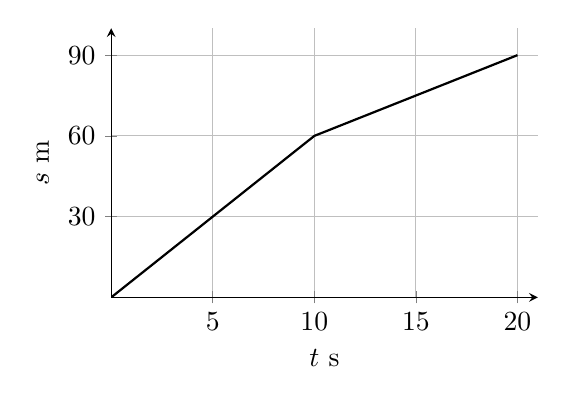
\begin{tikzpicture}
\begin{axis}[width=7cm,height=5cm,xmin=0,xmax=21,ymin=0,ymax=100,xtick={5,10,15,20},ytick={30,60,90},xlabel={$t$ s},ylabel={$s$ m},axis lines=left,grid=major]
\addplot[thick,black] coordinates {(0,0) (10,60) (20,90)};
\end{axis}
\end{tikzpicture}
\end{center}

\textbf{(c)} $v=6+4\mathrm{e}^{2t}$.

\textbf{(i)} $\mathrm{e}^{2t}>0$ for all $t$, so $v>6>0$: the velocity is never zero, so $R$ is never at rest.

\textbf{(ii)}
\[ a=\frac{\mathrm{d}v}{\mathrm{d}t}=8\mathrm{e}^{2t}=12 \;\Rightarrow\; \mathrm{e}^{2t}=\frac{3}{2} \;\Rightarrow\; \boxed{t=\frac{1}{2}\ln\frac{3}{2}} \]

\textbf{(iii)} Since $v>0$ throughout, the distance travelled is $\int v\,\mathrm{d}t$:
\[ s=\int_{0.4}^{0.5}\left(6+4\mathrm{e}^{2t}\right)\mathrm{d}t=\left[2\mathrm{e}^{2t}+6t\right]_{0.4}^{0.5} \]
\[ =\left(2\mathrm{e}+3\right)-\left(2\mathrm{e}^{0.8}+2.4\right)=8.436-6.851 \]
\[ \boxed{1.59\ \mathrm{m}} \]
\end{ansbox}

\end{document}
